\section{二代测序数据分析}
\subsection{常见术语}
\begin{frame}
  \frametitle{基因组学 | 数据分析 | 术语 | 深度 vs. 覆盖度}
  \begin{block}{深度(depth)}
    \begin{itemize}
      \item 也叫乘数,衡量测序量的首要参数;测序得到的总碱基数与待测基因组大小的比值;每个碱基被测序的平均次数
      \item 假设一个基因大小为2M,测序获得的总数据量为20M测序,那么深度为10X
    \end{itemize}
  \end{block}
  \pause
  \begin{block}{覆盖度(coverage)}
    \begin{itemize}
      \item 测序获得的序列占整个基因组的比例
      \item 由于基因组中的高GC、重复序列等复杂结构的存在,测序最终拼接组装获得的序列往往无法覆盖所有的区域,这部分没有获得的区域就称为Gap。例如一个细菌基因组测序,覆盖度是98\%,那么还有2\%的序列区域是没有通过测序获得的。
    \end{itemize}
  \end{block}
\end{frame}

\begin{frame}
  \frametitle{基因组学 | 数据分析 | 术语 | 深度 vs. 覆盖度}
  \begin{block}{实验}
对长100bp的目标区域进行捕获测序:采用单端测序,每个read长5bp;总共得到了200个reads;把所有的reads比对到目标区域后,100bp的目标区域中有98bp的位置至少有1个read覆盖到,换言之,剩余的2bp没有1个read覆盖。
  \end{block}
  \pause
  \begin{block}{深度与覆盖度}
    \begin{itemize}
      \item 深度:$200 \times 5 / 100 = 10$
      \item 覆盖度:$98 / 100 \times 100\% = 98\%$
    \end{itemize}
  \end{block}
\end{frame}

\begin{frame}
  \frametitle{基因组学 | 数据分析 | 术语 | SE vs. PE}
  \begin{figure}
    \centering
    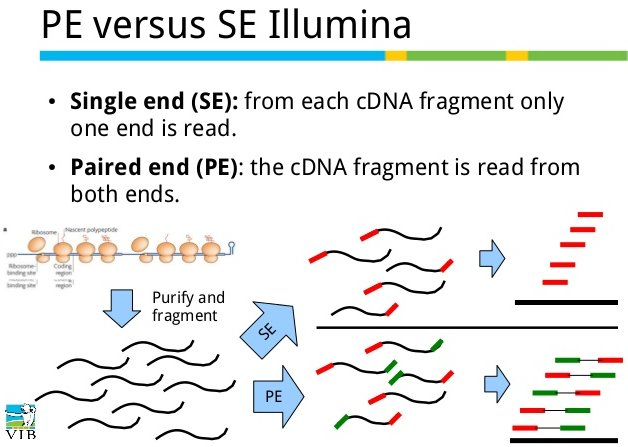
\includegraphics[width=0.85\textwidth]{c2.genomics/term.se.pe.01.jpg}
  \end{figure}
\end{frame}

\begin{frame}
  \frametitle{基因组学 | 数据分析 | 术语 | SE vs. PE}
  \begin{figure}
    \centering
    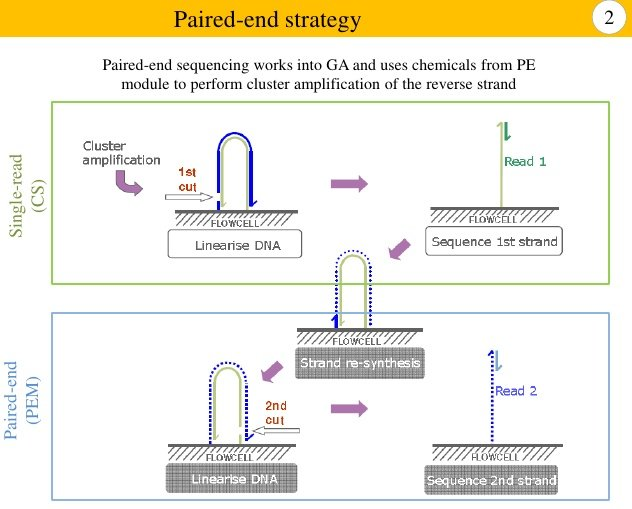
\includegraphics[width=0.8\textwidth]{c2.genomics/term.se.pe.02.jpg}
  \end{figure}
\end{frame}

\begin{frame}
  \frametitle{基因组学 | 数据分析 | 术语 | PE}
  \begin{block}{Paired-End Sequencing}
    \begin{itemize}
      \item allows users to sequence both ends of a fragment and generate high-quality, alignable sequence data
      \item facilitates detection of genomic rearrangements and repetitive sequence elements, as well as gene fusions and novel transcripts
    \end{itemize}
  \end{block}
  \begin{figure}
    \centering
    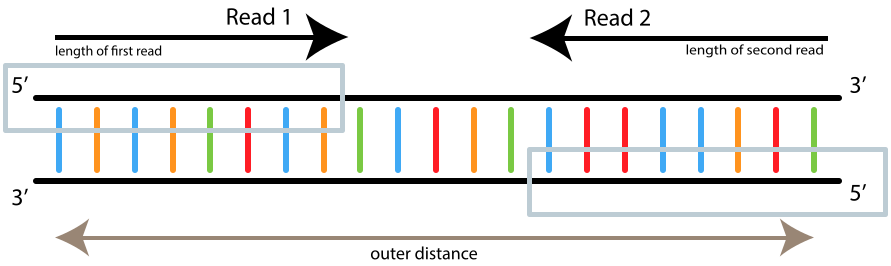
\includegraphics[width=0.9\textwidth]{c2.genomics/term.pe.01.png}
  \end{figure}
\end{frame}

\begin{frame}
  \frametitle{基因组学 | 数据分析 | 术语 | PE}
  \begin{block}{Paired-End DNA Sequencing}
    \begin{itemize}
      \item provide superior alignment across DNA regions containing repetitive sequences
      \item produce longer contigs for de novo sequencing by filling gaps in the consensus sequence
      \item detect rearrangements such as insertions, deletions, and inversions
    \end{itemize}
  \end{block}
  \pause
  \begin{block}{Paired-End RNA Sequencing}
    \begin{itemize}
      \item enable discovery applications such as detecting gene fusions in cancer and characterizing novel splice isoforms.
    \end{itemize}
  \end{block}
\end{frame}

\begin{frame}
  \frametitle{基因组学 | 数据分析 | 术语 | PE}
  \begin{figure}
    \centering
    \only<1->{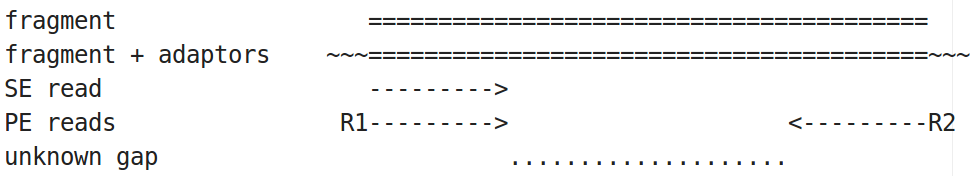
\includegraphics[width=\textwidth]{c2.genomics/term.insert.size.01.png}}\\
    \vspace{1em}
    \only<2->{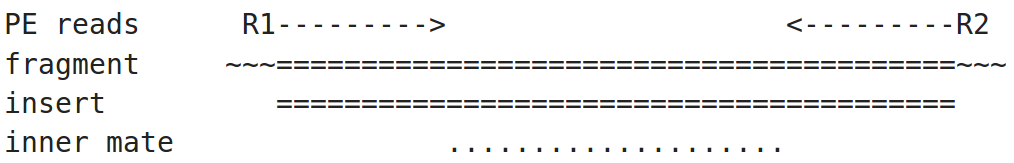
\includegraphics[width=\textwidth]{c2.genomics/term.insert.size.02.png}}
  \end{figure}
  \only<3->{
  \begin{block}{Conclusion}
Remember that ``insert" refers to the DNA fragment between the adaptors, and not the gap between R1 and R2. Instead we refer to that as the ``inner mate distance".
  \end{block}
  }
\end{frame}

\begin{frame}
  \frametitle{基因组学 | 数据分析 | 术语 | 其他}
  \begin{figure}
    \centering
    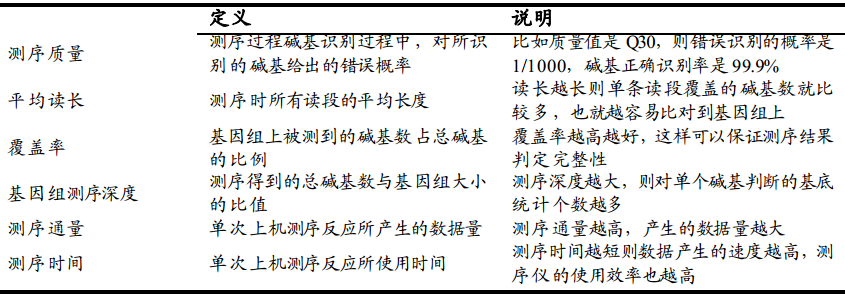
\includegraphics[width=\textwidth]{c2.genomics/term.other.01.png}
  \end{figure}
\end{frame}

\subsection{分析流程}
\begin{frame}
  \frametitle{基因组学 | 数据分析 | 流程 | 概述 | 总览}
  \begin{figure}
    \centering
    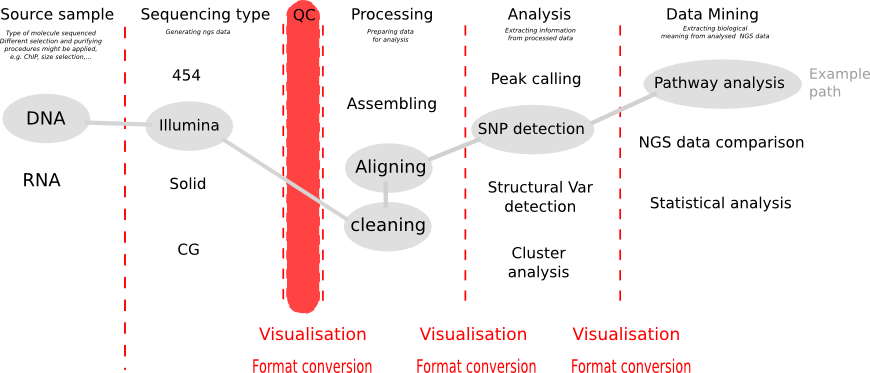
\includegraphics[width=\textwidth]{c2.genomics/workflow.ngs.05.png}
  \end{figure}
\end{frame}

\begin{frame}
  \frametitle{基因组学 | 数据分析 | 流程 | 概述 | 总览}
  \begin{figure}
    \centering
    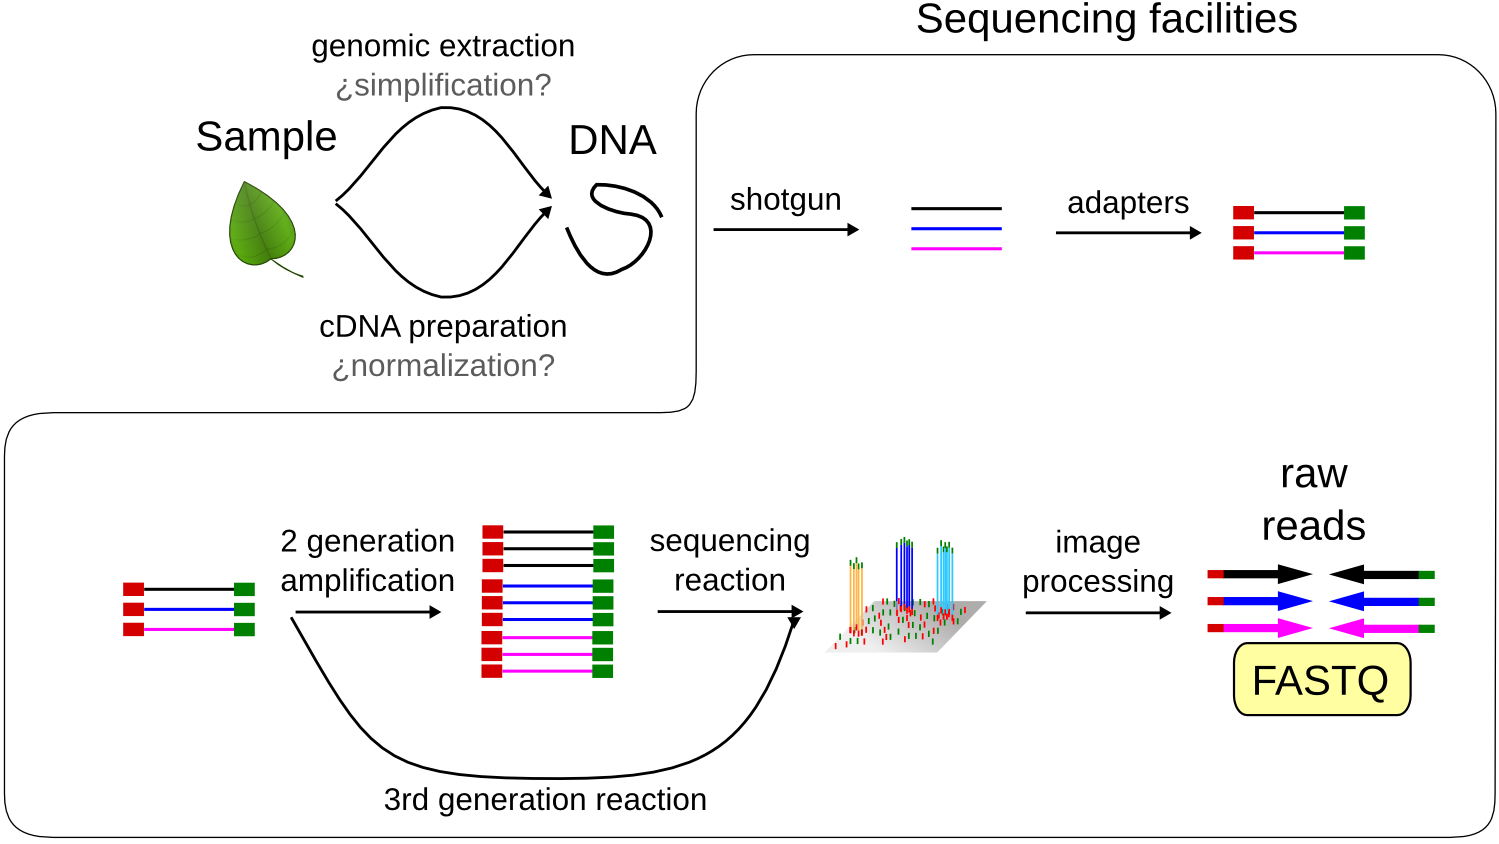
\includegraphics[width=\textwidth]{c2.genomics/workflow.ngs.01.png}
  \end{figure}
\end{frame}

\begin{frame}
  \frametitle{基因组学 | 数据分析 | 流程 | 概述 | 总览}
  \begin{figure}
    \centering
    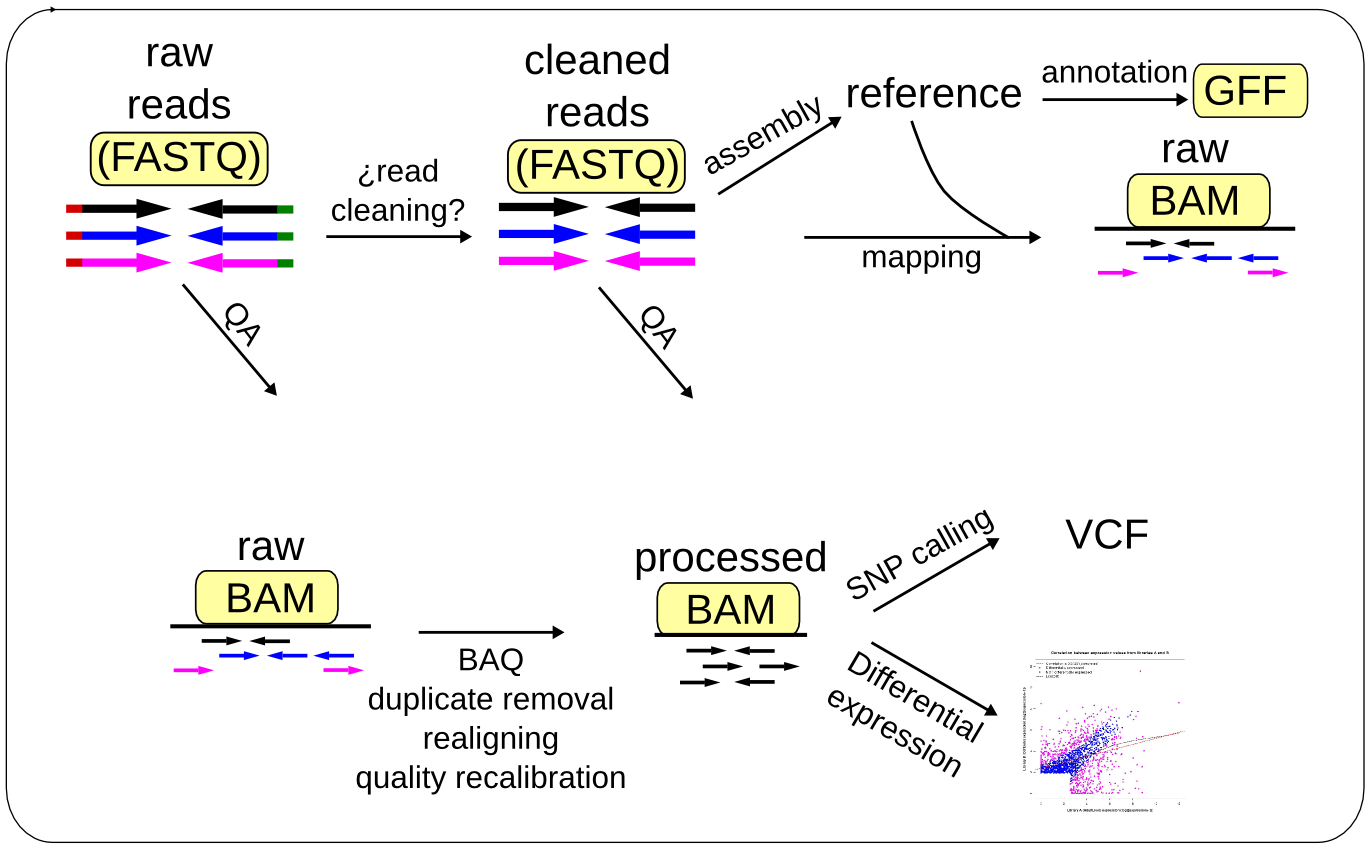
\includegraphics[width=\textwidth]{c2.genomics/workflow.ngs.02.png}
  \end{figure}
\end{frame}

\begin{frame}
  \frametitle{基因组学 | 数据分析 | 流程 | 概述 | Seqs}
  \begin{figure}
    \centering
    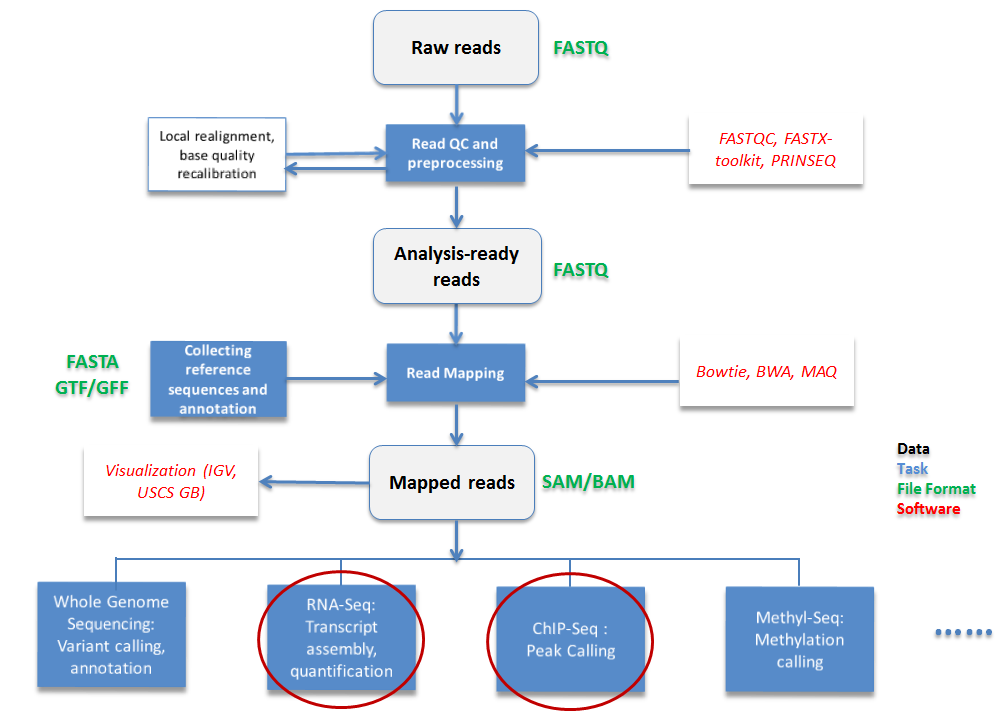
\includegraphics[width=0.9\textwidth]{c2.genomics/workflow.ngs.03.png}
  \end{figure}
\end{frame}

\begin{frame}
  \frametitle{基因组学 | 数据分析 | 流程 | 概述 | Seqs}
  \begin{figure}
    \centering
    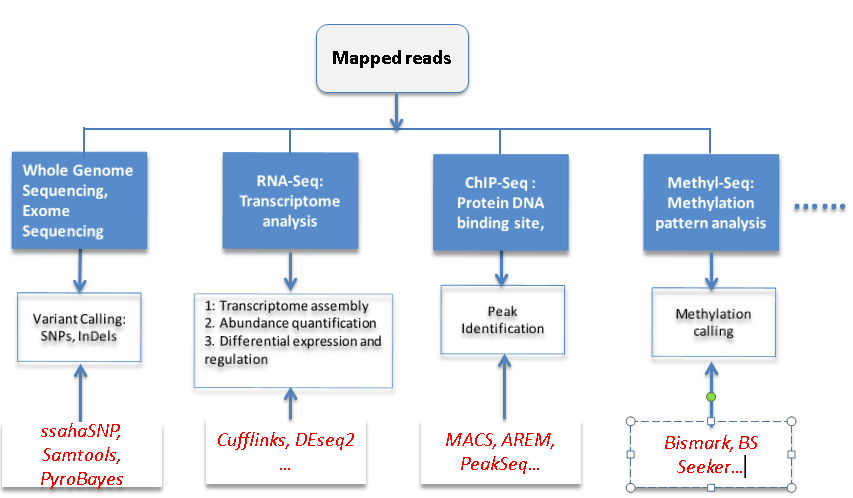
\includegraphics[width=\textwidth]{c2.genomics/workflow.ngs.04.png}
  \end{figure}
\end{frame}

\begin{frame}
  \frametitle{基因组学 | 数据分析 | 流程 | 概述 | 总览}
  \begin{figure}
    \centering
    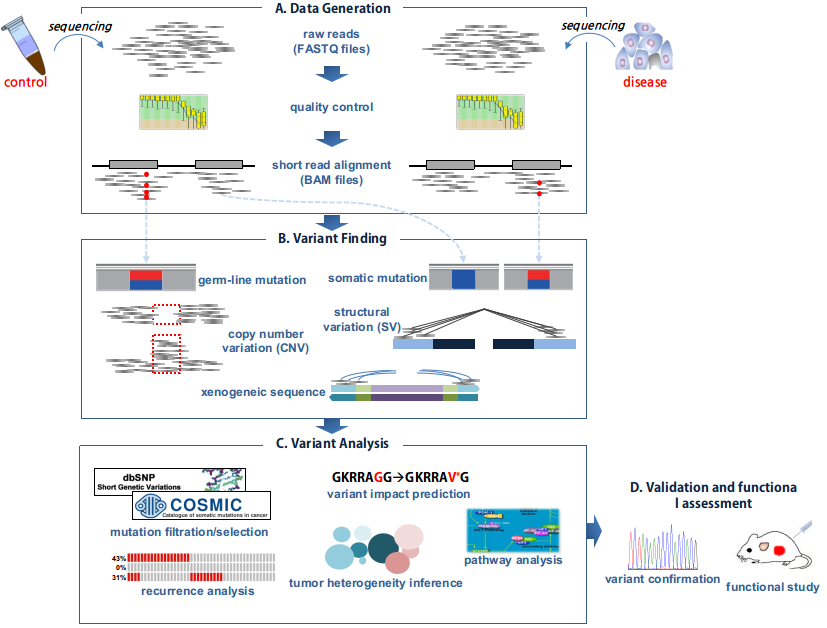
\includegraphics[width=0.85\textwidth]{c2.genomics/workflow.ngs.10.png}
  \end{figure}
\end{frame}

\begin{frame}
  \frametitle{基因组学 | 数据分析 | 流程 | 概述 | Exome}
  \begin{figure}
    \centering
    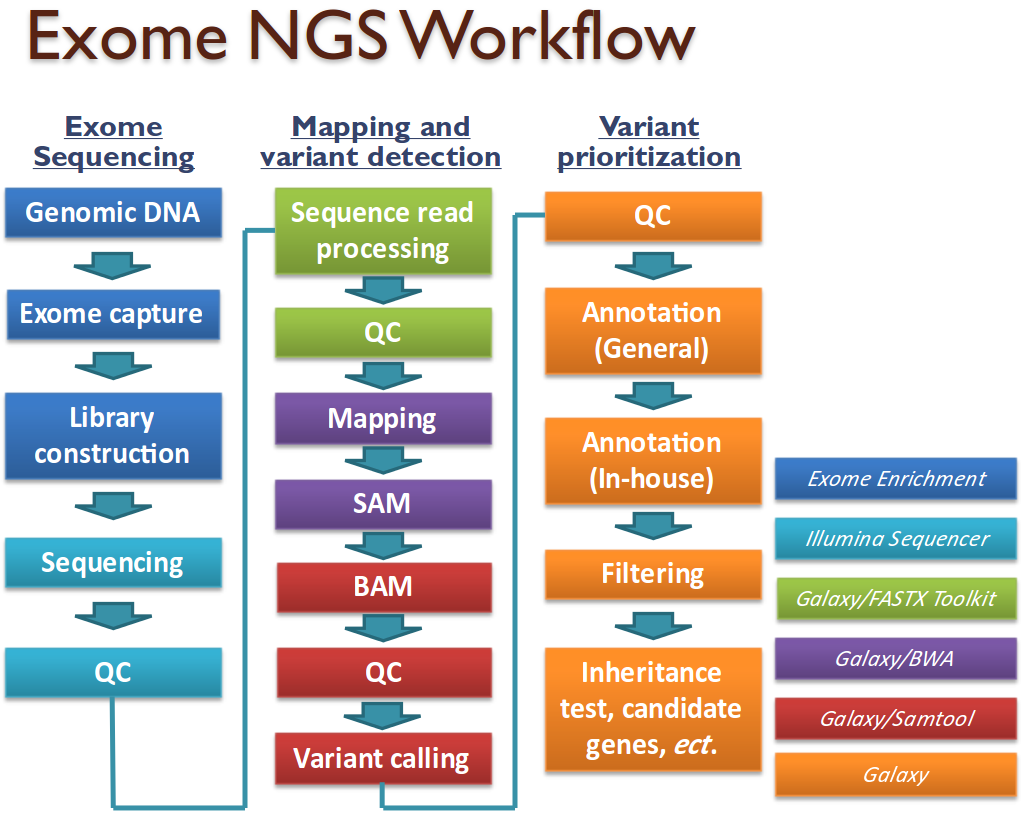
\includegraphics[width=0.9\textwidth]{c2.genomics/workflow.exome.03.png}
  \end{figure}
\end{frame}

\begin{frame}
  \frametitle{基因组学 | 数据分析 | 流程 | 质控(Quality Control)}
  \begin{figure}
    \centering
    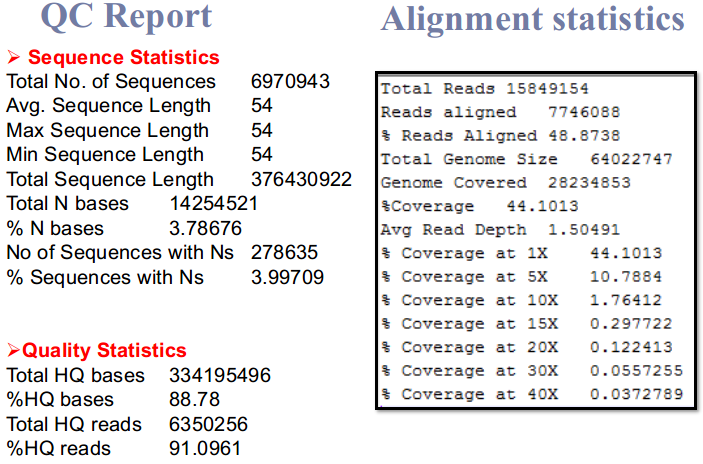
\includegraphics[width=0.9\textwidth]{c2.genomics/qc.report.01.png}
  \end{figure}
\end{frame}

\begin{frame}
  \frametitle{基因组学 | 数据分析 | 流程 | 质控 | 工具}
  \begin{figure}
    \centering
    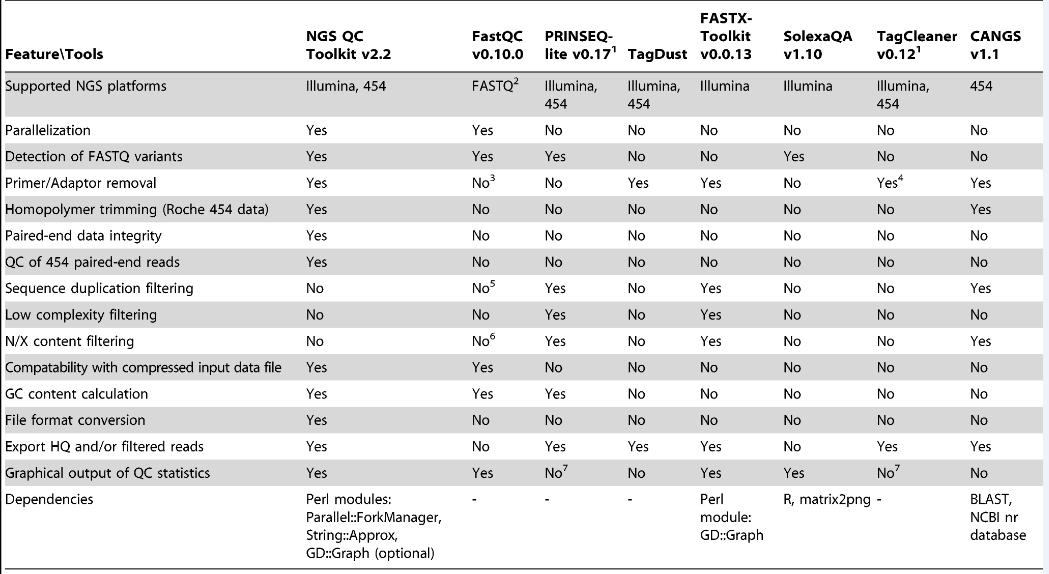
\includegraphics[width=\textwidth]{c2.genomics/qc.tool.01.png}
  \end{figure}
\end{frame}

\begin{frame}
  \frametitle{基因组学 | 数据分析 | 流程 | 质控 | 工具}
  \begin{block}{FastQC}
    A quality control tool for high throughput sequence data.
  \end{block}
  \pause
  \begin{block}{NGS QC Toolkit}
    A toolkit for the quality control (QC) of next generation sequencing (NGS) data.
  \end{block}
  \pause
  \begin{block}{Others}
    \begin{itemize}
      \item SolexaQA: calculates sequence quality statistics and creates visual representations of data quality for second-generation sequencing data.
      \item ...
    \end{itemize}
  \end{block}
\end{frame}

\begin{frame}
  \frametitle{基因组学 | 数据分析 | 流程 | 质控 | FastQC}
  \begin{figure}
    \centering
    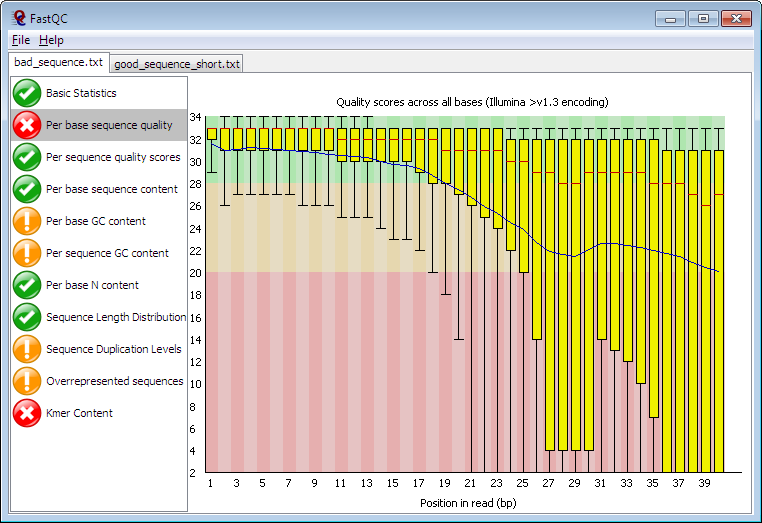
\includegraphics[width=0.9\textwidth]{c2.genomics/qc.fastqc.01.png}
  \end{figure}
\end{frame}

\begin{frame}
  \frametitle{基因组学 | 数据分析 | 流程 | 质控 | FastQC}
  \begin{figure}
    \centering
    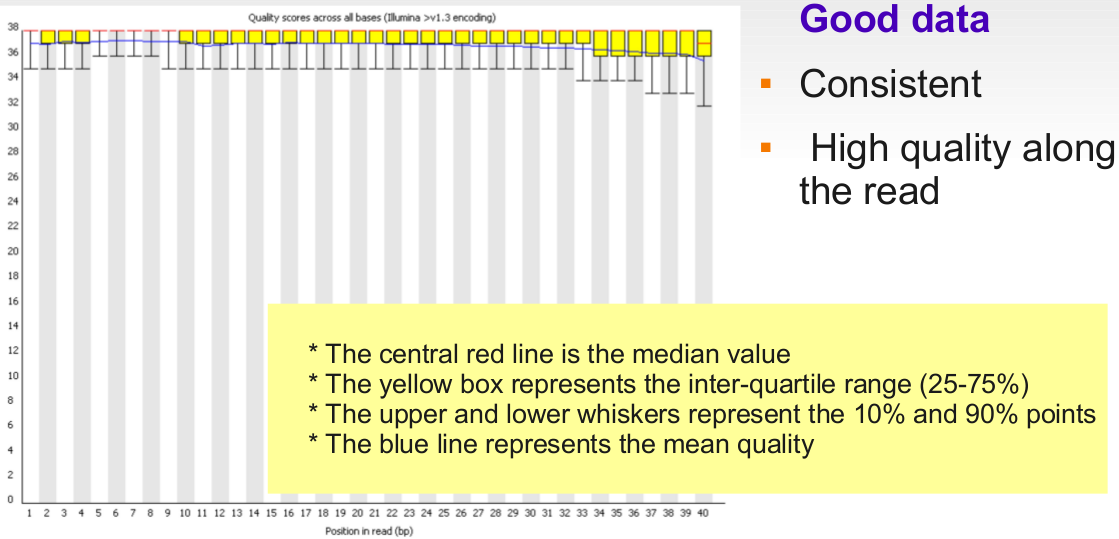
\includegraphics[width=\textwidth]{c2.genomics/qc.fastqc.10.png}
  \end{figure}
\end{frame}

\begin{frame}
  \frametitle{基因组学 | 数据分析 | 流程 | 质控 | FastQC}
  \begin{figure}
    \centering
    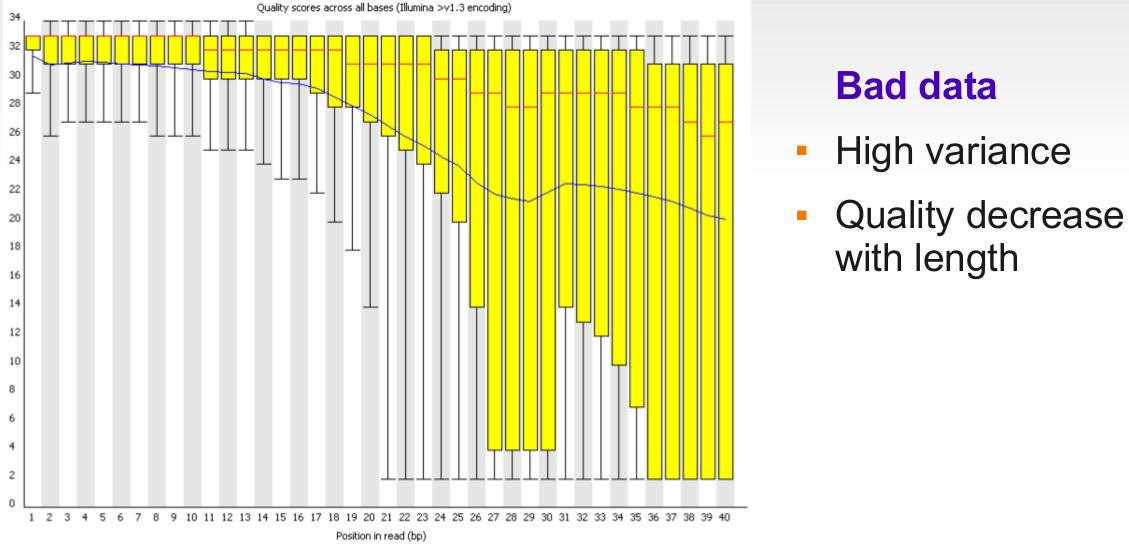
\includegraphics[width=\textwidth]{c2.genomics/qc.fastqc.11.png}
  \end{figure}
\end{frame}

\begin{frame}
  \frametitle{基因组学 | 数据分析 | 流程 | 质控 | FastQC}
  \begin{figure}
    \centering
    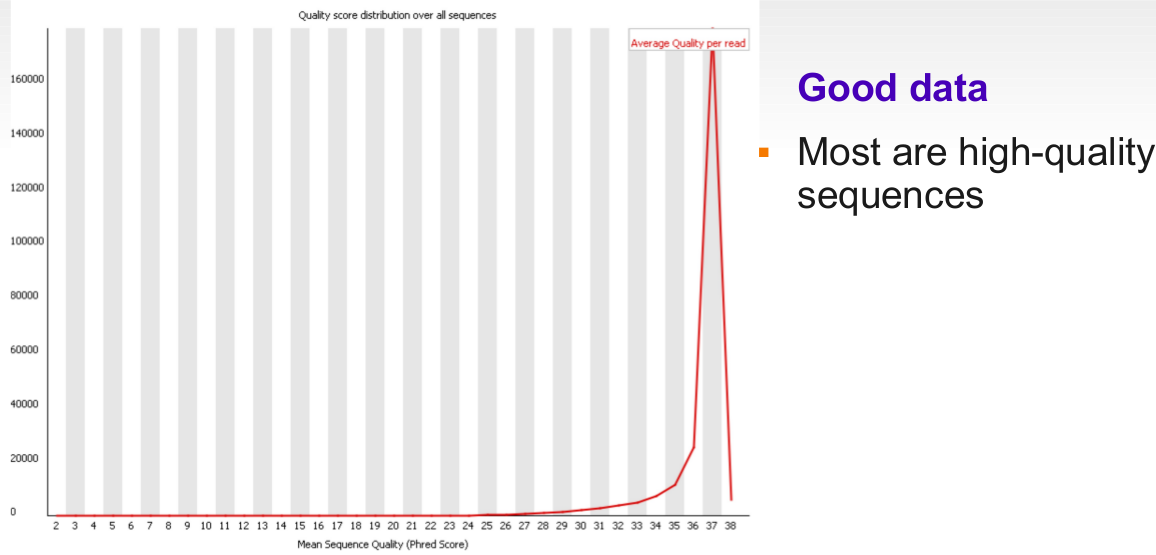
\includegraphics[width=\textwidth]{c2.genomics/qc.fastqc.12.png}
  \end{figure}
\end{frame}

\begin{frame}
  \frametitle{基因组学 | 数据分析 | 流程 | 质控 | FastQC}
  \begin{figure}
    \centering
    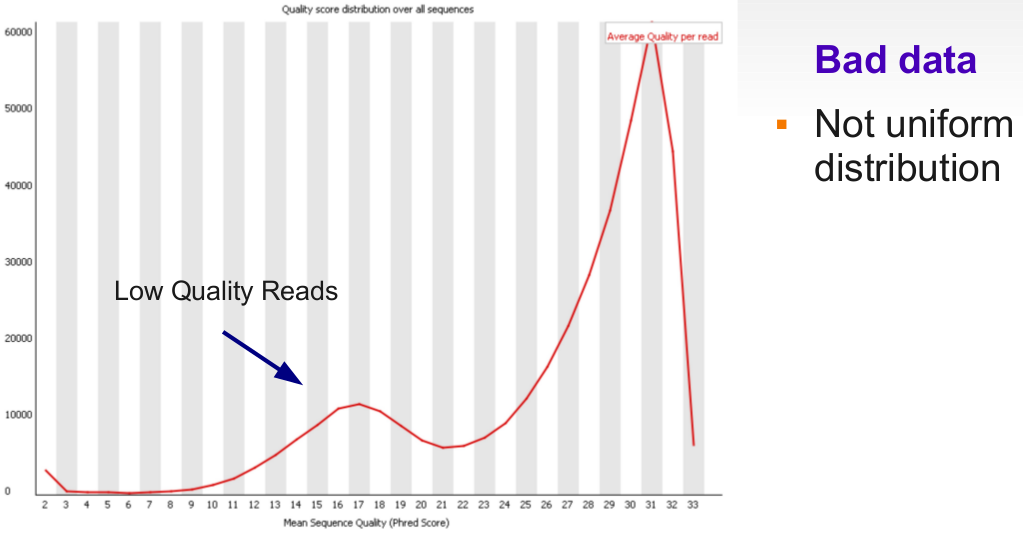
\includegraphics[width=\textwidth]{c2.genomics/qc.fastqc.13.png}
  \end{figure}
\end{frame}

\begin{frame}
  \frametitle{基因组学 | 数据分析 | 流程 | 质控 | FastQC}
  \begin{figure}
    \centering
    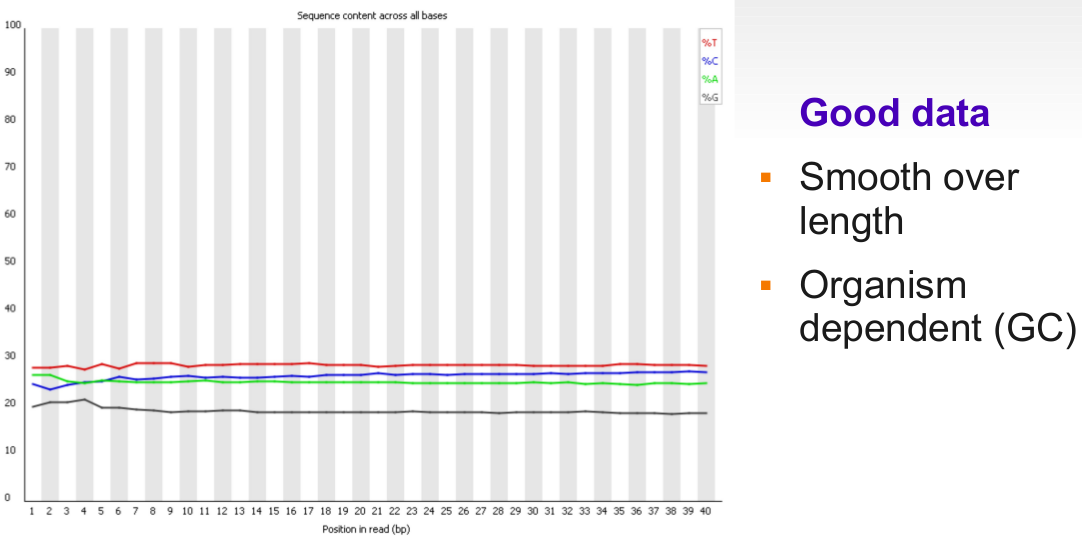
\includegraphics[width=\textwidth]{c2.genomics/qc.fastqc.14.png}
  \end{figure}
\end{frame}

\begin{frame}
  \frametitle{基因组学 | 数据分析 | 流程 | 质控 | FastQC}
  \begin{figure}
    \centering
    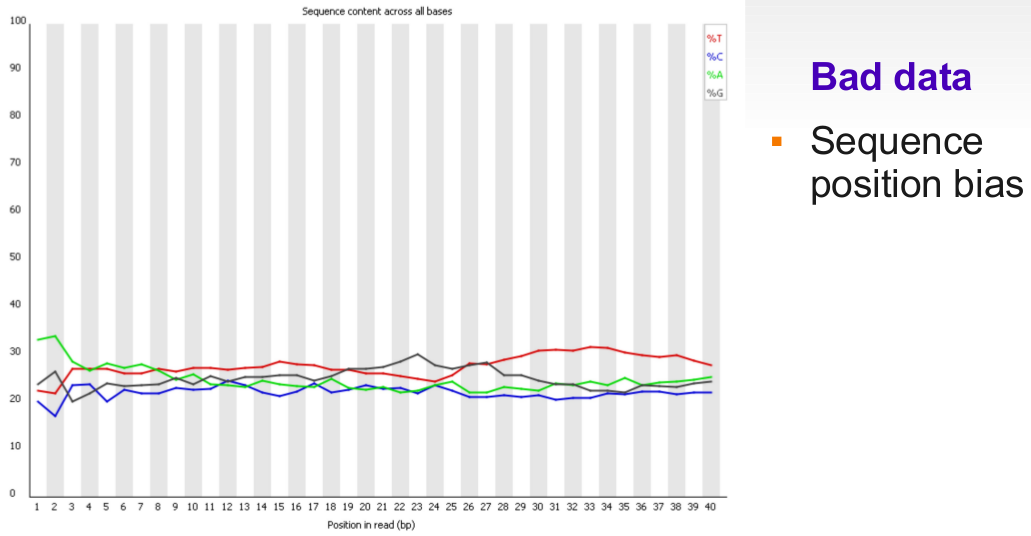
\includegraphics[width=\textwidth]{c2.genomics/qc.fastqc.15.png}
  \end{figure}
\end{frame}

\begin{frame}
  \frametitle{基因组学 | 数据分析 | 流程 | 质控 | FastQC}
  \begin{figure}
    \centering
    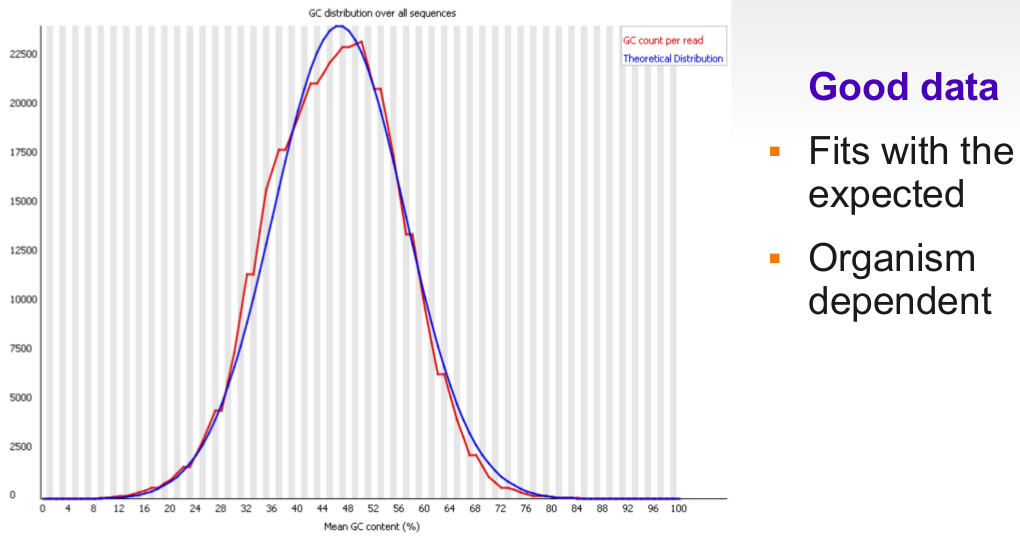
\includegraphics[width=\textwidth]{c2.genomics/qc.fastqc.16.png}
  \end{figure}
\end{frame}

\begin{frame}
  \frametitle{基因组学 | 数据分析 | 流程 | 质控 | FastQC}
  \begin{figure}
    \centering
    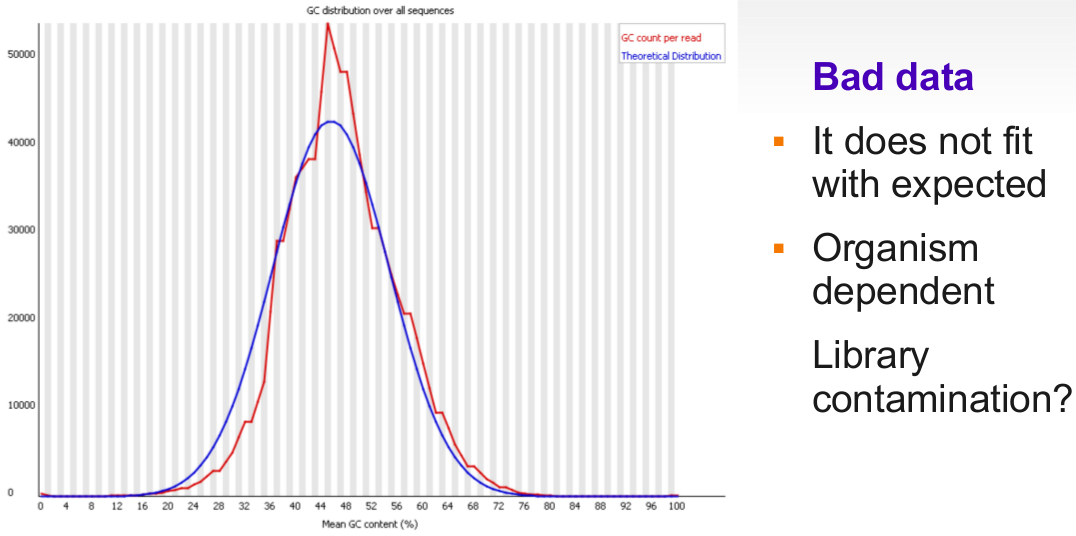
\includegraphics[width=\textwidth]{c2.genomics/qc.fastqc.17.png}
  \end{figure}
\end{frame}

\begin{frame}
  \frametitle{基因组学 | 数据分析 | 流程 | 质控 | FastQC}
  \begin{figure}
    \centering
    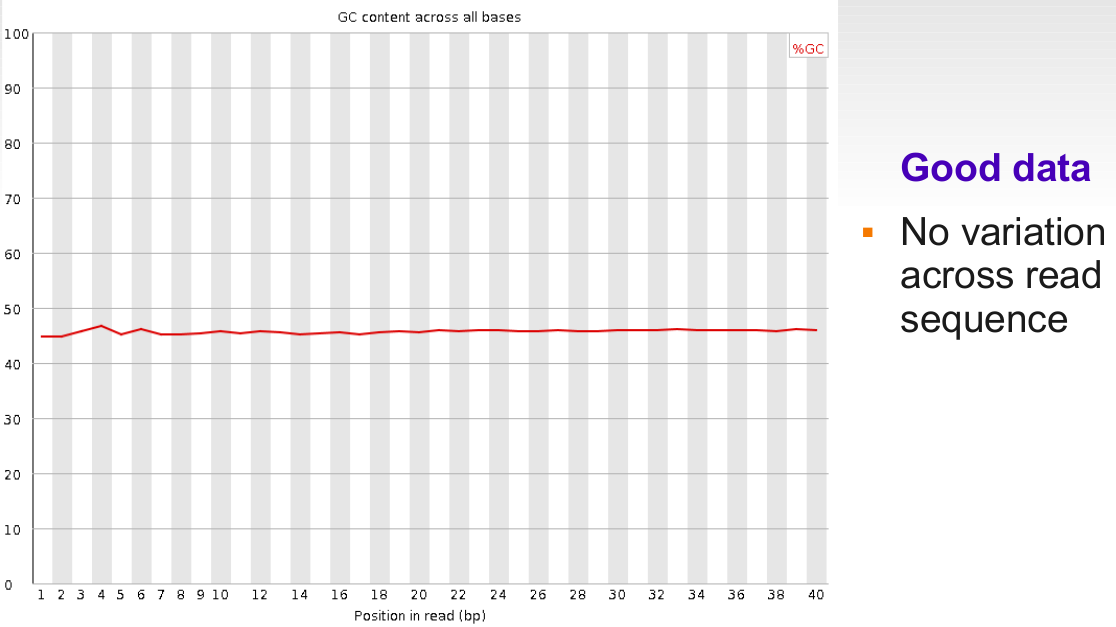
\includegraphics[width=\textwidth]{c2.genomics/qc.fastqc.18.png}
  \end{figure}
\end{frame}

\begin{frame}
  \frametitle{基因组学 | 数据分析 | 流程 | 质控 | FastQC}
  \begin{figure}
    \centering
    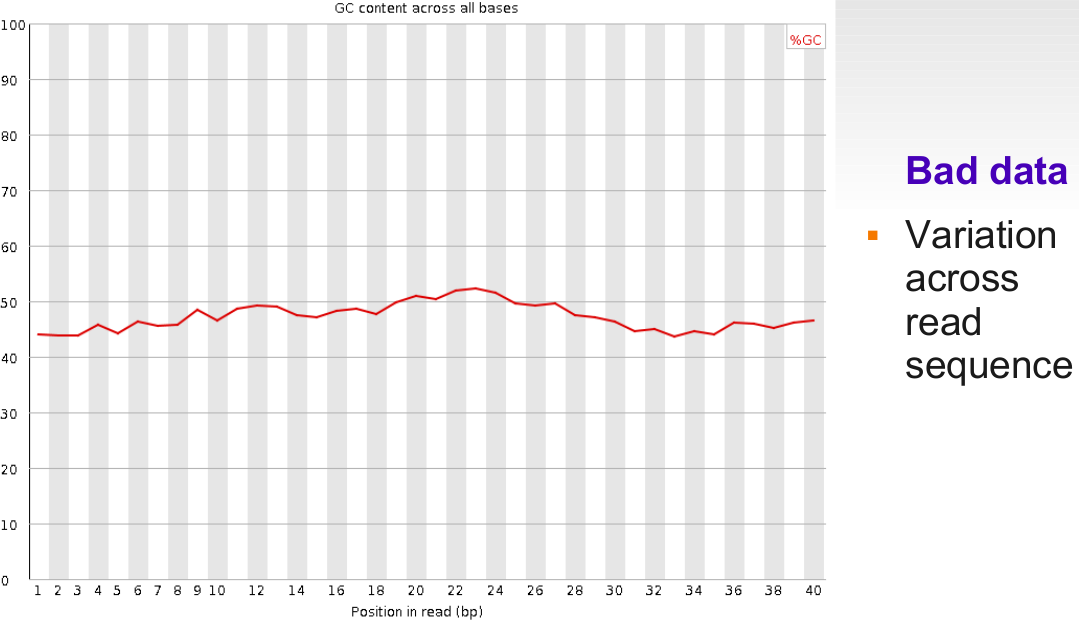
\includegraphics[width=\textwidth]{c2.genomics/qc.fastqc.19.png}
  \end{figure}
\end{frame}

\begin{frame}
  \frametitle{基因组学 | 数据分析 | 流程 | 质控 | FastQC}
  \begin{figure}
    \centering
    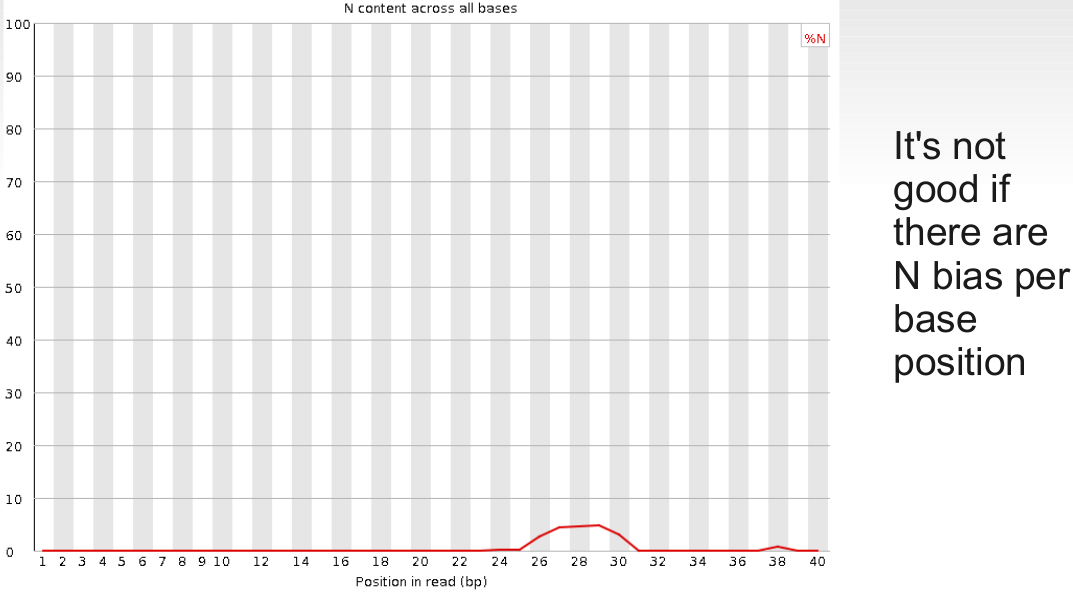
\includegraphics[width=\textwidth]{c2.genomics/qc.fastqc.20.png}
  \end{figure}
\end{frame}

\begin{frame}
  \frametitle{基因组学 | 数据分析 | 流程 | 质控 | FastQC}
  \begin{figure}
    \centering
    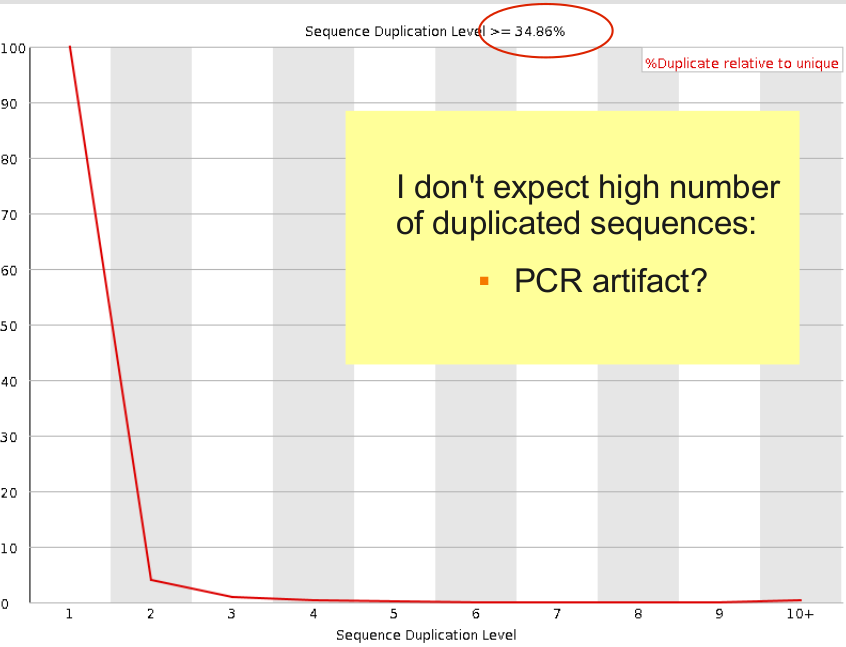
\includegraphics[width=0.85\textwidth]{c2.genomics/qc.fastqc.21.png}
  \end{figure}
\end{frame}

\begin{frame}
  \frametitle{基因组学 | 数据分析 | 流程 | 质控 | FastQC}
  \begin{figure}
    \centering
    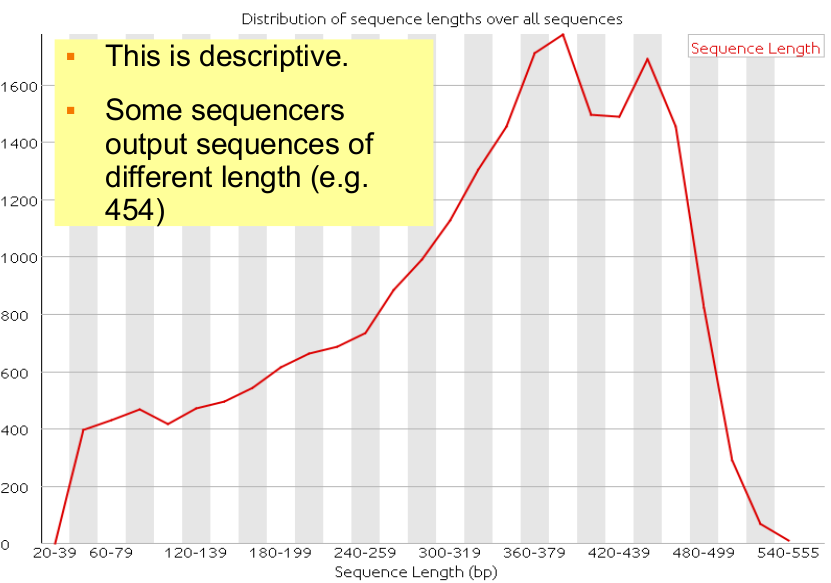
\includegraphics[width=0.9\textwidth]{c2.genomics/qc.fastqc.22.png}
  \end{figure}
\end{frame}

\begin{frame}
  \frametitle{基因组学 | 数据分析 | 流程 | 质控 | FastQC}
  \begin{figure}
    \centering
    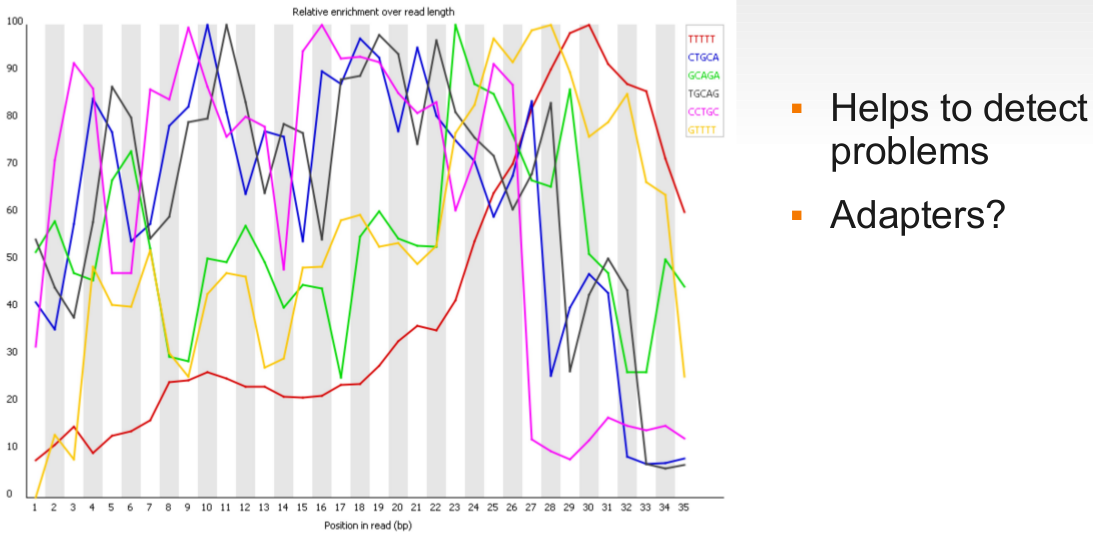
\includegraphics[width=\textwidth]{c2.genomics/qc.fastqc.23.png}
  \end{figure}
\end{frame}

\begin{frame}
  \frametitle{基因组学 | 数据分析 | 流程 | 质控 | NGS QC Toolkit}
  \begin{figure}
    \centering
    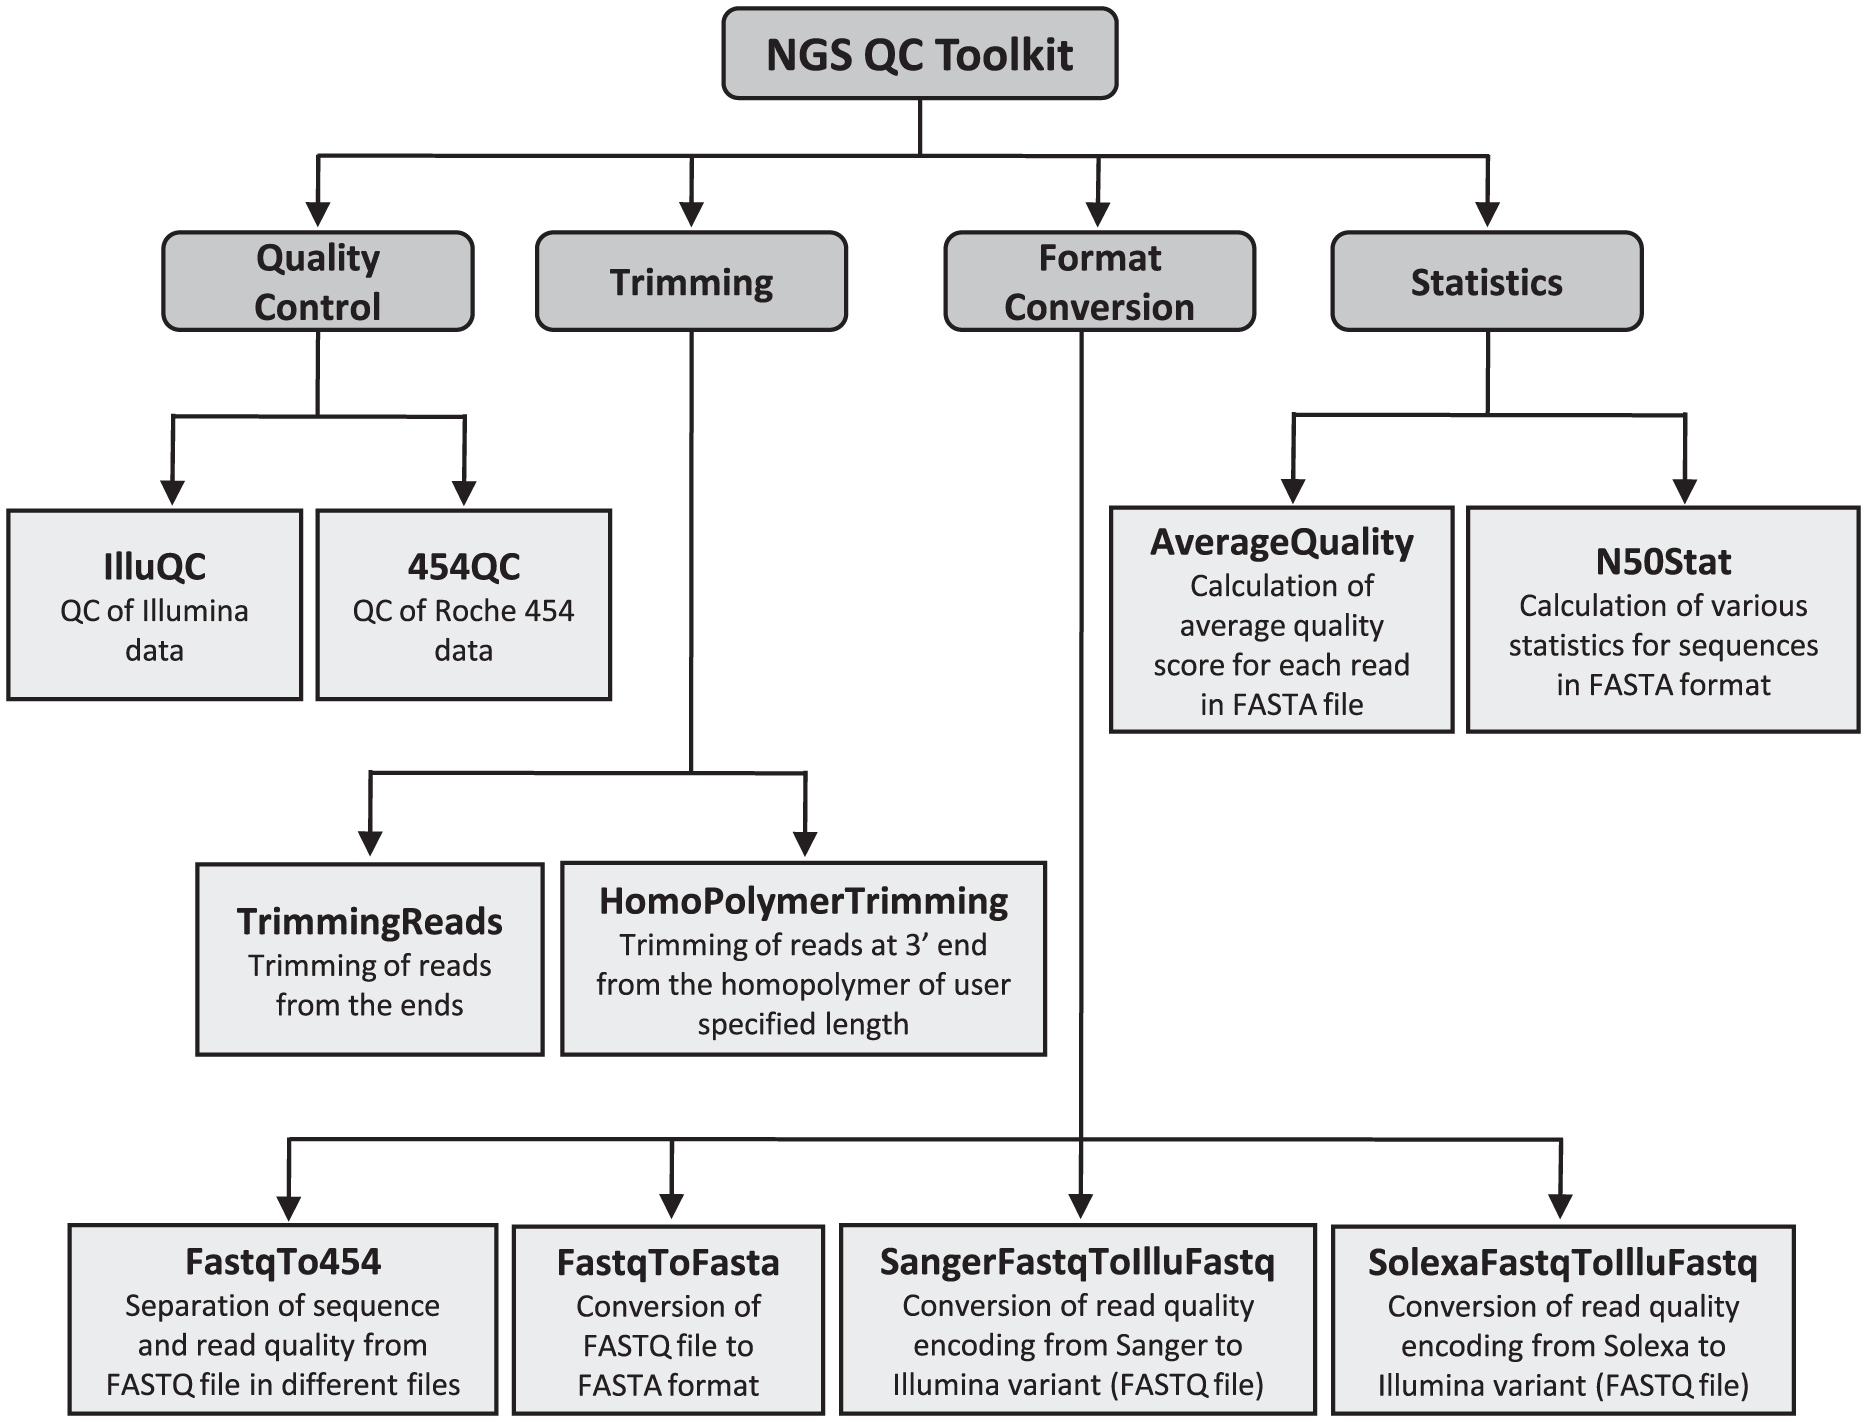
\includegraphics[width=0.8\textwidth]{c2.genomics/qc.ngs.01.png}
  \end{figure}
\end{frame}

\begin{frame}
  \frametitle{基因组学 | 数据分析 | 流程 | 质控 | NGS QC Toolkit}
  \begin{figure}
    \centering
    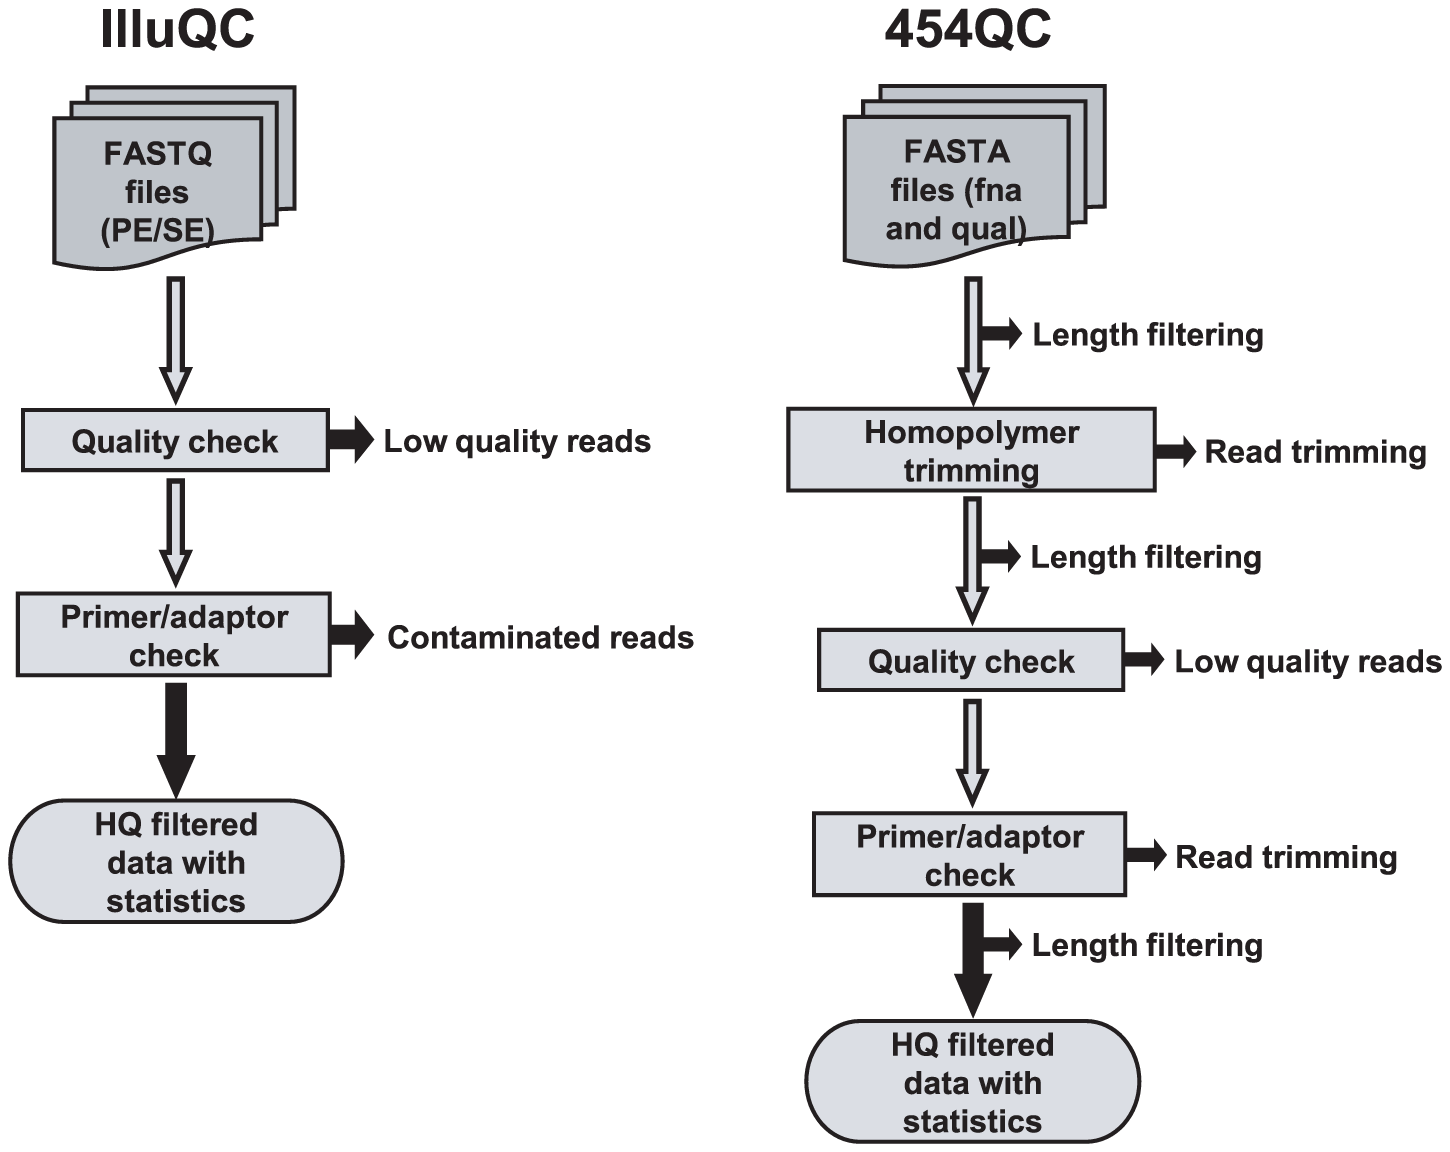
\includegraphics[width=0.8\textwidth]{c2.genomics/qc.ngs.02.png}
  \end{figure}
\end{frame}

\begin{frame}
  \frametitle{基因组学 | 数据分析 | 流程 | 质控 | NGS QC Toolkit}
  \begin{figure}
    \centering
    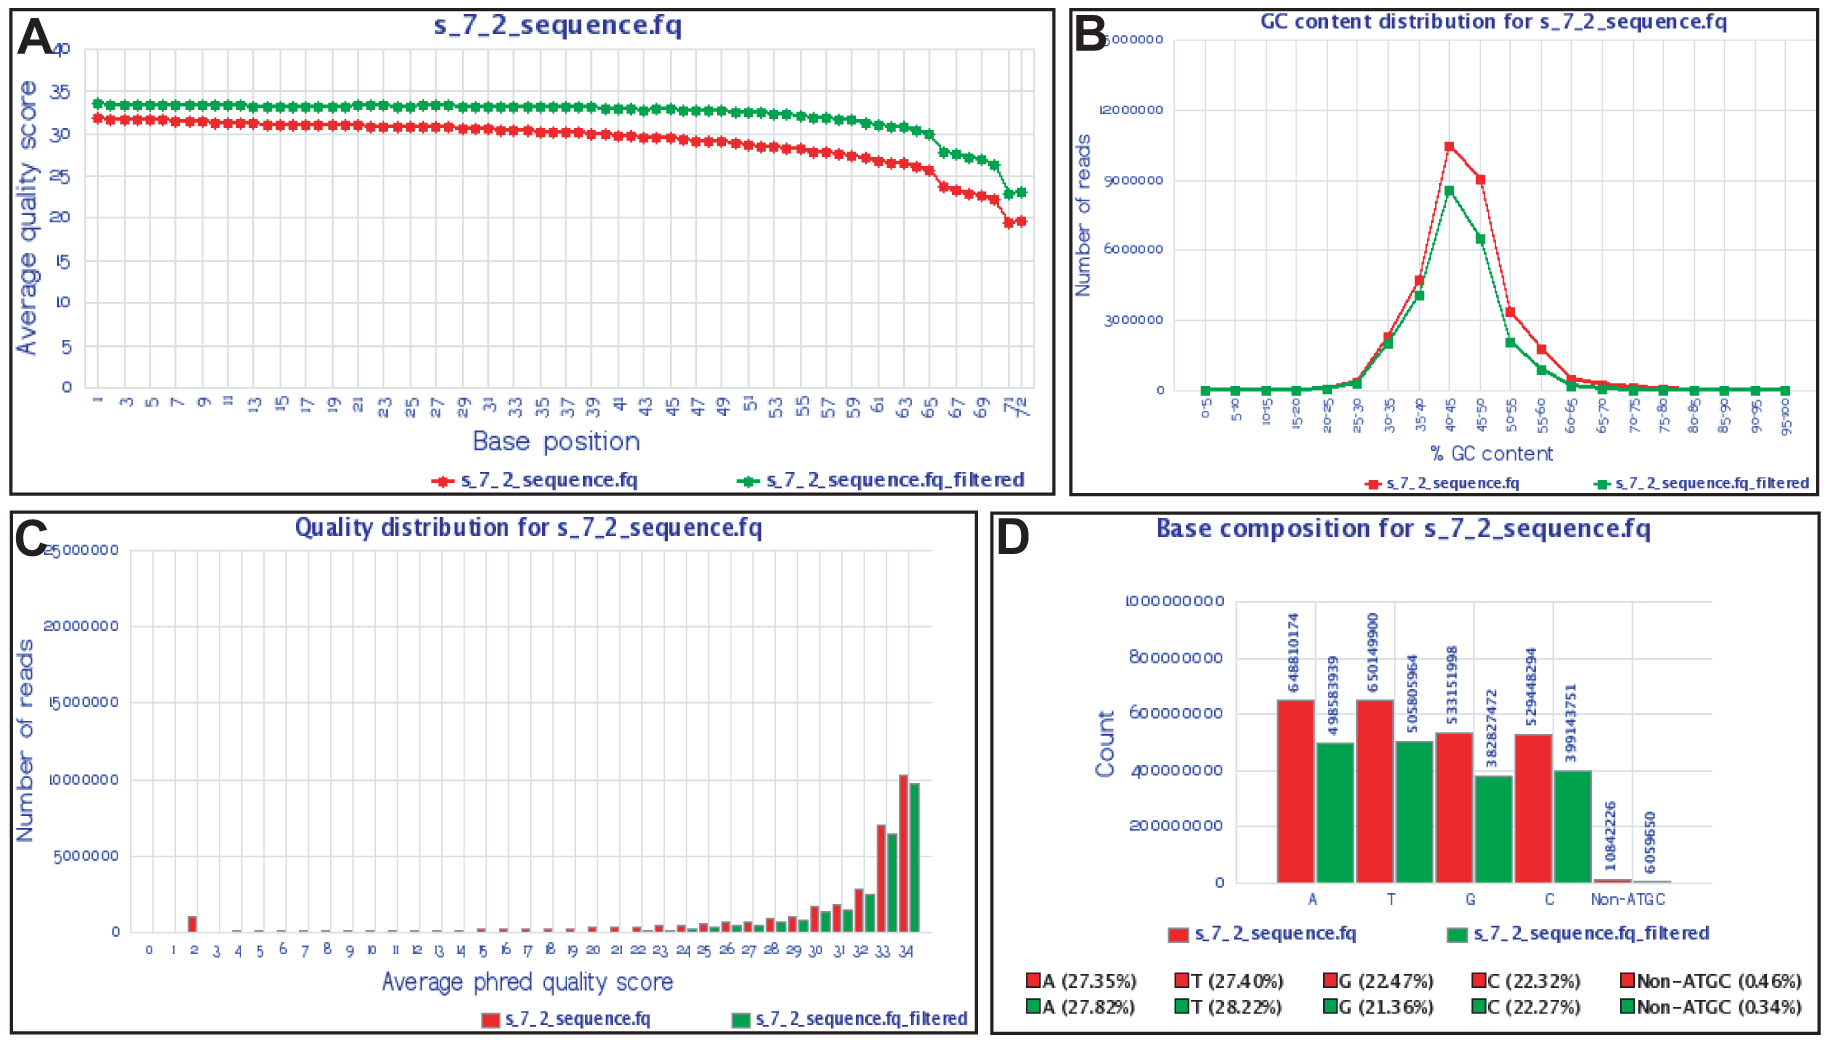
\includegraphics[width=\textwidth]{c2.genomics/qc.ngs.03.png}
  \end{figure}
\end{frame}

\begin{frame}
  \frametitle{基因组学 | 数据分析 | 流程 | 质控 | NGS QC Toolkit}
  \begin{figure}
    \centering
    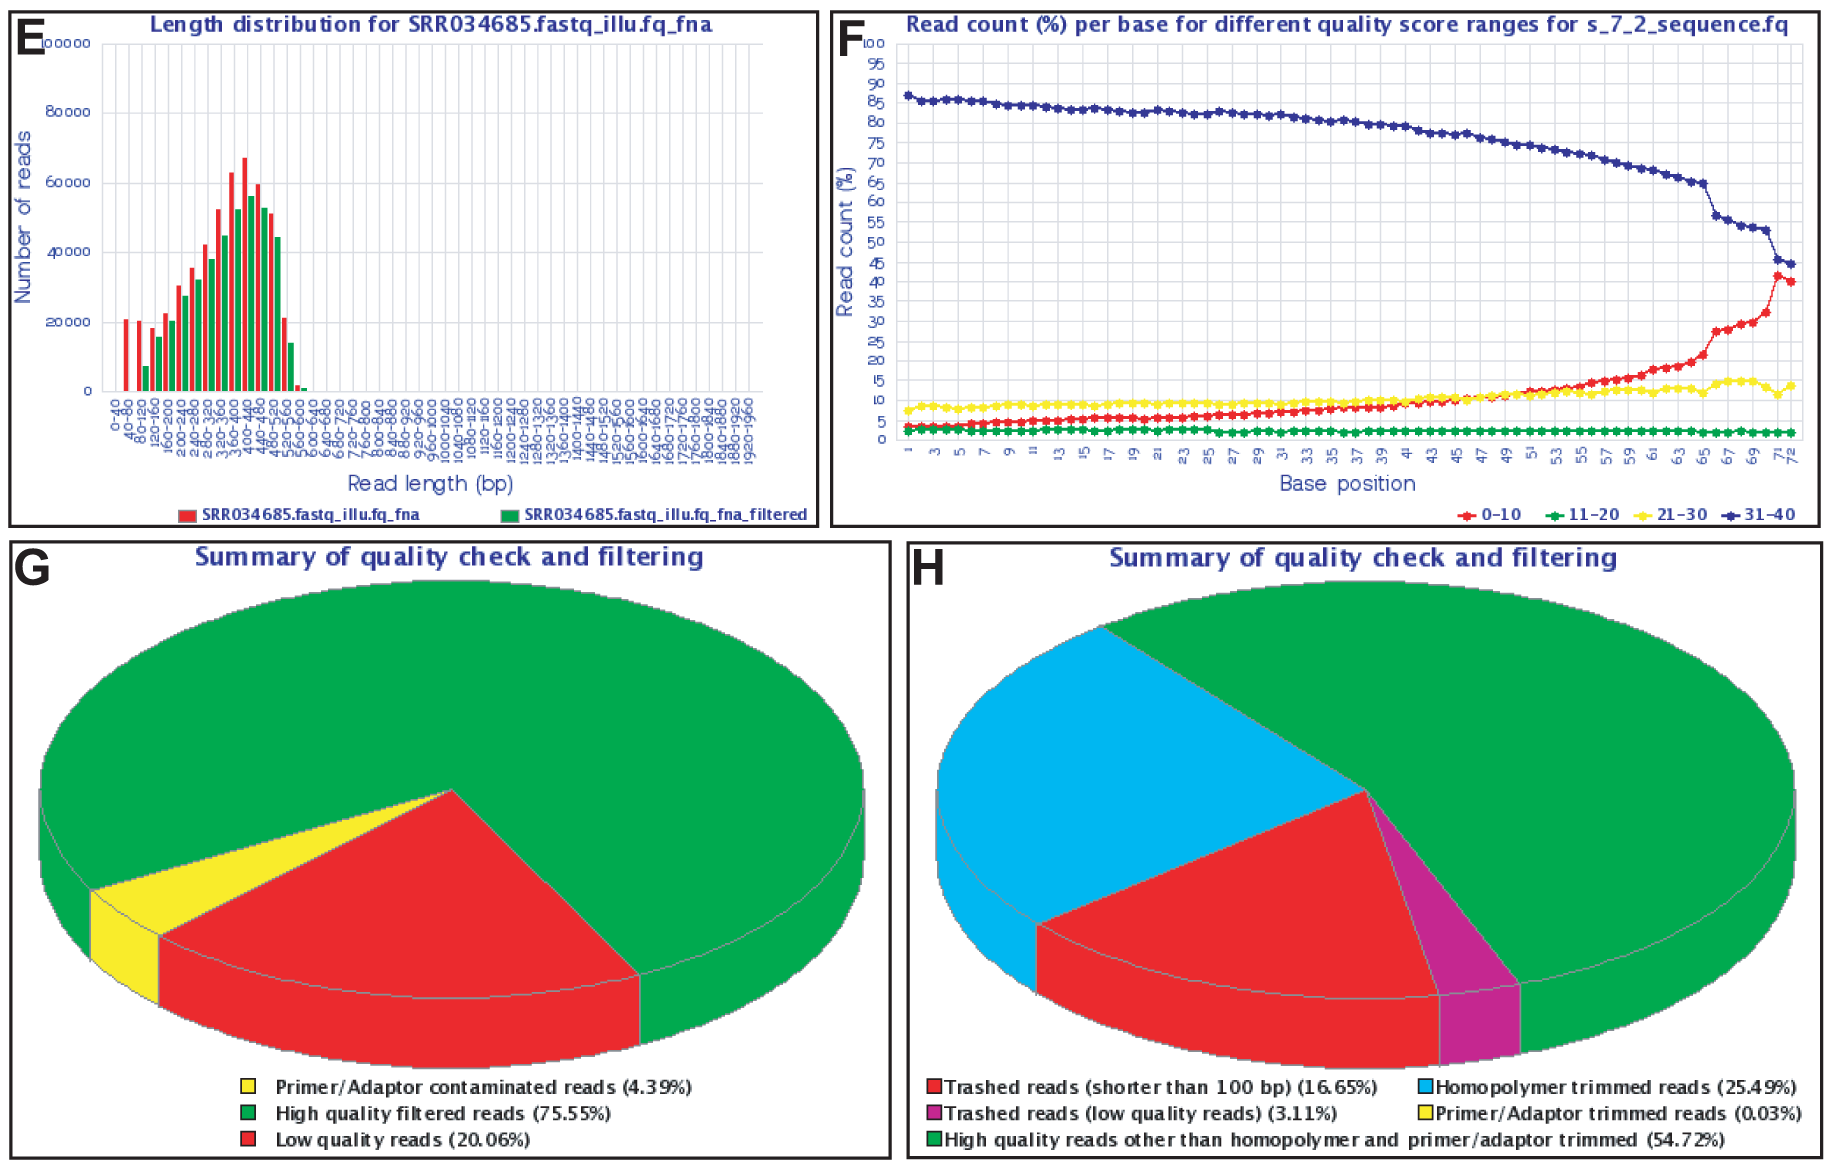
\includegraphics[width=\textwidth]{c2.genomics/qc.ngs.04.png}
  \end{figure}
\end{frame}

\begin{frame}
  \frametitle{基因组学 | 数据分析 | 流程 | 质控 | SolexaQA}
  \begin{figure}
    \centering
    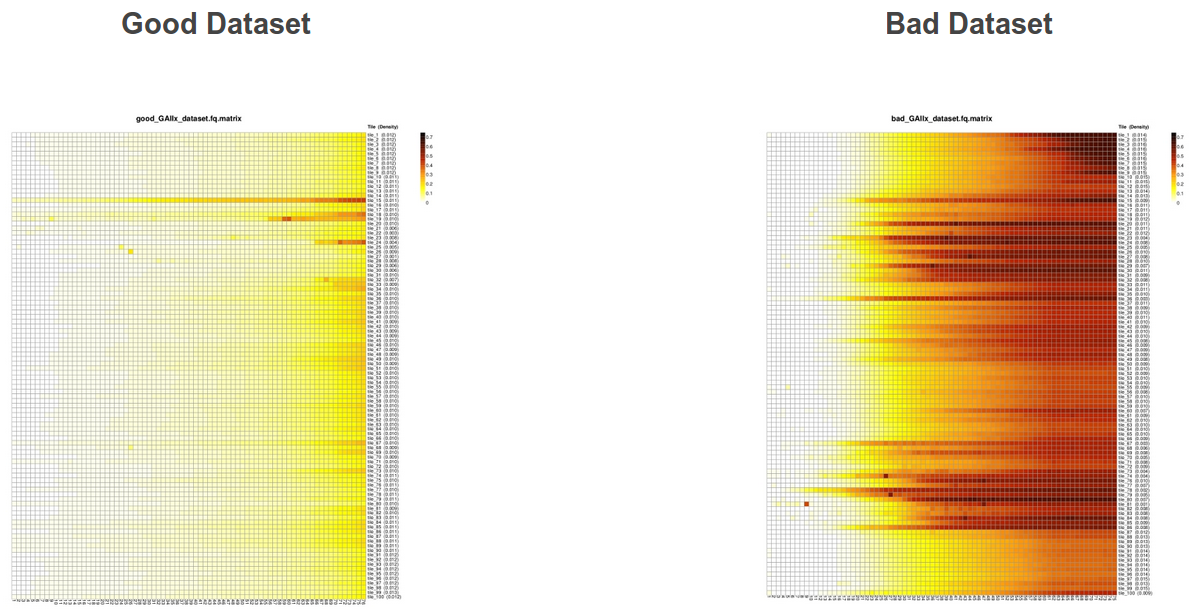
\includegraphics[width=\textwidth]{c2.genomics/qc.qa.01.png}
  \end{figure}
\end{frame}

\begin{frame}
  \frametitle{基因组学 | 数据分析 | 流程 | 质控 | SolexaQA}
  \begin{figure}
    \centering
    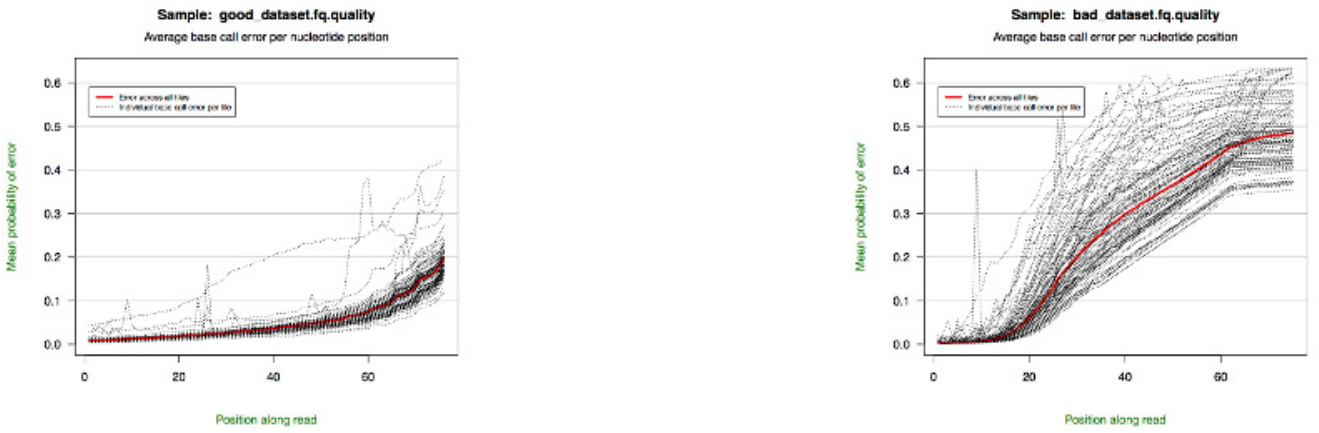
\includegraphics[width=\textwidth]{c2.genomics/qc.qa.02.png}
  \end{figure}
\end{frame}

\begin{frame}
  \frametitle{基因组学 | 数据分析 | 流程 | 质控 | SolexaQA}
  \begin{figure}
    \centering
    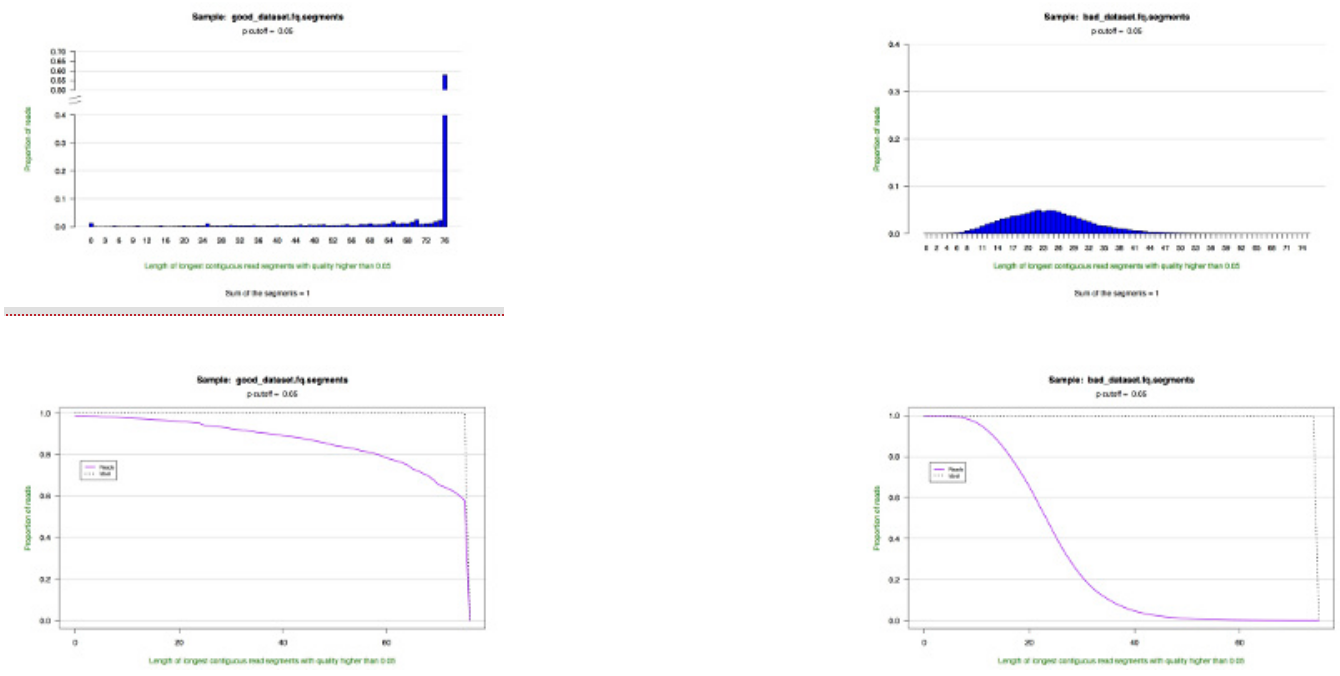
\includegraphics[width=\textwidth]{c2.genomics/qc.qa.03.png}
  \end{figure}
\end{frame}

\begin{frame}
  \frametitle{基因组学 | 数据分析 | 流程 | 预处理}
\end{frame}

\begin{frame}
  \frametitle{基因组学 | 数据分析 | 流程 | 预处理 | 工具}
  \begin{block}{}
  \end{block}
  \pause
  \begin{block}{PRINSEQ}
    A publicly available tool that is able to filter, reformat and trim your sequences and to provide you summary statistics for your sequence data.
  \end{block}
  \pause
  \begin{block}{}
  \end{block}
\end{frame}

\begin{frame}
  \frametitle{基因组学 | 数据分析 | 流程 | 预处理}
\end{frame}


\begin{frame}[label=current]
  \frametitle{基因组学 | 数据分析 | 流程 | 比对}
\end{frame}

\begin{frame}[label=current]
  \frametitle{基因组学 | 数据分析 | 流程 | 寻找变异}
\end{frame}

\begin{frame}[label=current]
  \frametitle{基因组学 | 数据分析 | 流程 | 注释变异}
\end{frame}

\begin{frame}[label=current]
  \frametitle{基因组学 | 数据分析 | 流程 | 可视化}
\end{frame}

